\section{Success criteria}

Referring to the~\nameref{ch:proposal}, I met all success criteria of the project


\begin{todolist}
    \item[\done] Implemented the experimental framework (\graffs) to automate experiments of robustness of graph metrics
    \item[\done] Completed statistical analysis and compared results to The Paper
    \item[\done] Extended the idea from The Paper to unscored networks, and deduced empirical observations about graph metrics on interesting unscored datasets
\end{todolist}

For the evaluation of \graffs, I designed the following experiments:
\begin{description}
    \item[\texttt{reproduce}] focuses on reproducing some results from The Paper, following the setup from The Paper as closely as possible
    \item[\texttt{random-edges}] validates whether random edge deletion is a suitable graph generation method, by applying the same pipeline as in \texttt{repr} just with random edge deletion
    \item[\texttt{unscored}] applies the random edge deletion method to new, unscored, datasets
\end{description}

In analyses in the following sections, the protein network datasets \texttt{pvivax}, \texttt{ecoli}, \texttt{yeast} are the exact datasets that were used in The Paper\footnote{The datasets are available at \url{https://github.com/lbozhilova/measuring_rank_robustness}}.
They originate from the STRING database, but the database changes over time, so to validate \graffs by reproducing the results I preferred using the same datasets over their new version.


\section{Validation against The Paper}

One of the added values of \graffs is the ability to experiment with \textsl{unscored} graphs.
However, in order to validate whether the results produced by \graffs are legit, I first constructed and ran a \texttt{reproduce} experiment trying to reproduce results from The Paper, by linearly thresholding 3 scored protein interaction networks in the same way as The Paper.

The \texttt{reproduce} experiment with the \texttt{thMedHigh} generator (producing 31 graphs at linearly spaced thresholds between 0.60 and 0.90 confidence values) were set up in the following way:
% @formatter:off
\begin{lstlisting}[language=bash]
graffs dataset download-demos
graffs generator create --name thMedHigh --method threshold-linear --params 600,900 -n 31 --seed 7
graffs experiment create --name reproduce --datasets pvivax,ecoli,yeast --generator thMedHigh --metrics Betweenness,Degree,Ego1Edges,Ego2Nodes,LocalClustering,PageRank,Redundancy --robustnessMeasures RankIdentifiability,RankInstability,RankContinuity
graffs experiment run --name reproduce
\end{lstlisting}
% @formatter:on

As for the set of metrics, I evaluated all that were also evaluated in The Paper, apart from Closeness and Harmonic centrality (Definitions~\ref{def:closeness_centrality} and~\ref{def:harmonic_centrality}).
These two depend on the all pair shortest paths algorithm with time complexity $O({\left\lvert V \right\rvert}^3)$ that would take unreasonable amount of time to compute on large graphs. (\todo{evaluating Closeness on one graph takes XY minutes\ldots})

It is important to note that the robustness values from The Paper and \graffs should not be compared directly as there are many details that make the numerical values vary between implementations.
For example, when ranking nodes according to a metric, The Paper resolved ties randomly for each perturbed graph (which already leads to fluctuations in rankings), while my implementation resolves ties arbitrarily but predictably and constantly across all perturbed graphs of a dataset, with the purpose to improve reliability of robustness measures.
The Paper also randomly resolved ties when calculating the overall ranking (Definition~\ref{def:overall_ranking}).
Furthermore, there are other nuances that may cause these variations, such as $\alpha,k$ coefficients used for $k$-similarity and $\alpha$-relaxed $k$-similarity (different values were used in \graffs to generalize the process; see definitions~\ref{def:k_similarity},~\ref{def:alpha_relaxed_k_similarity}), definitions of graph metrics in special cases (such as for isolated nodes), and floating-point arithmetic.

\begin{figure}
    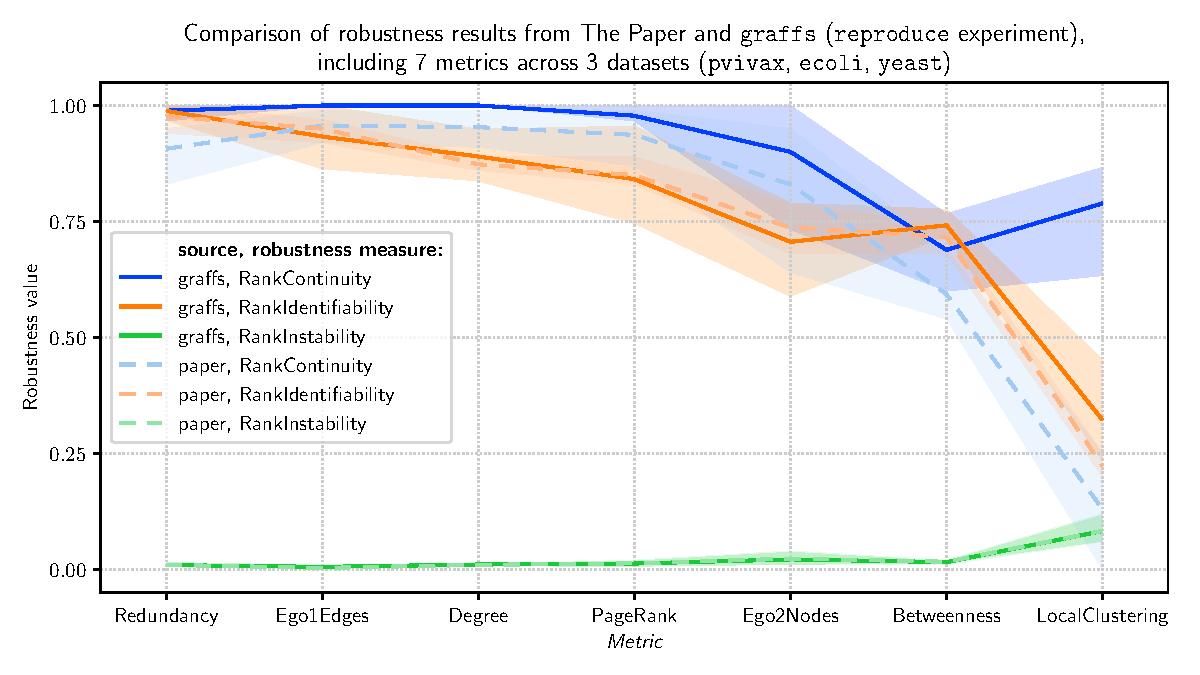
\includegraphics[width=\linewidth]{plot_reproduction.pdf}
    \caption{Comparison of results from The Paper and \graffs.
    Each color corresponds to one robustness measure, with thin lines inside each band showing robustness of individual datasets, and the thick line showing the average robustness across the 3 datasets.
    Solid and dashed bands correspond to results obtained by \graffs and The Paper, respectively.}
    \label{fig:plot_reproduction}
    \footnotesize
    \begin{flushleft}
        Note that high values of RankContinuity and RankIdentifiability mean high \textsl{robustness}, whereas high values of RankInstability mean low \textsl{robustness}.
        Metrics are sorted from left to right by their decreasing combined robustness.
    \end{flushleft}
\end{figure}


Averaging the robustness values across the 3 protein datasets with similar structure (namely \texttt{pvivax}, \texttt{ecoli}, \texttt{yeast}), \autoref{fig:plot_reproduction} demonstrates that \graffs is successful in identifying similar robustness properties of metrics as in The Paper.
The Paper identifies metrics \texttt{Ego1Edges}, \texttt{Redundancy}, \texttt{Ego2Nodes}, \texttt{Degree} as very stable (i.e. robust).
Those have reported RankContinuity and RankIdentifiability values above $0.75$ on almost all evaluations on the 3 datasets, and RankInstability below $\sim 0.1$.
\graffs also reports these metrics as relatively stable, although the RankIdentifiability value is lower in general.

On the other hand, \texttt{Betweenness} and \texttt{LocalClustering} are considered unstable by The Paper (RankContinuity and RankIdentifiability significantly dropped while RankInstability increased), and the results from \graffs copy the behaviour.
Although the RankContinuity values of \texttt{LocalClustering} are not as low as reported by The Paper, one can definitely conclude that these two metrics are equally identified as less robust by \graffs.

For further thought, we can also consider variance of robustness measures, concluding, for example, that \texttt{Redundancy} (a stable metric) has small variance in RankIdentifiability across the 3 datasets, whereas the RankContinuity and RankIdentifiability of the \texttt{Ego2Nodes} metric led to more diverse values.

\subsection{Rank similarity}

Another way to validate intermediate results is to consider $k$-similarity of perturbed graphs between two consecutive thresholds, and $\alpha$-relaxed $k$-similarity between graphs at individual thresholds and overall ranks.
For each dataset \texttt{pvivax}, \texttt{ecoli}, \texttt{yeast}, I generated $85$ graphs thresholded at values between $0.15$ and $0.99$, and calculated the needed metric values for each graph.
Then I compare the results for 3 chosen metrics on the protein network datasets with the results of The Paper.

\begin{figure}
    \begin{enumerate}
        \item[(a)] 
\includegraphics[scale=1.05]{plot_rank_similarity_papertop.pdf}\\
        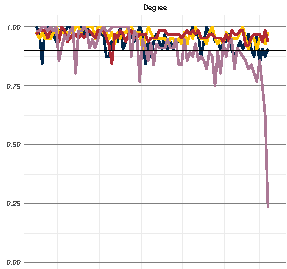
\includegraphics[scale=1.05]{plot_rank_similarity_paper_degree.pdf}\hspace*{0.1mm}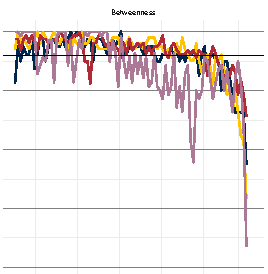
\includegraphics[scale=1.05]{plot_rank_similarity_paper_betweenness.pdf}\hspace*{-0.4mm}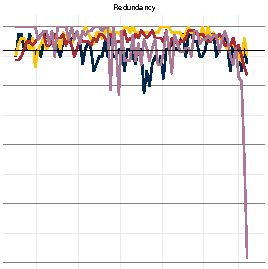
\includegraphics[scale=1.05]{plot_rank_similarity_paper_redundancy.pdf}\\
        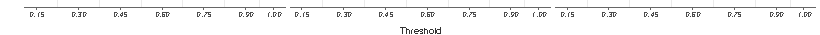
\includegraphics[scale=1.05]{plot_rank_similarity_paperbottom.pdf}
        \vspace*{-0.6cm}
        \item[(b)] \hspace*{-0.25cm}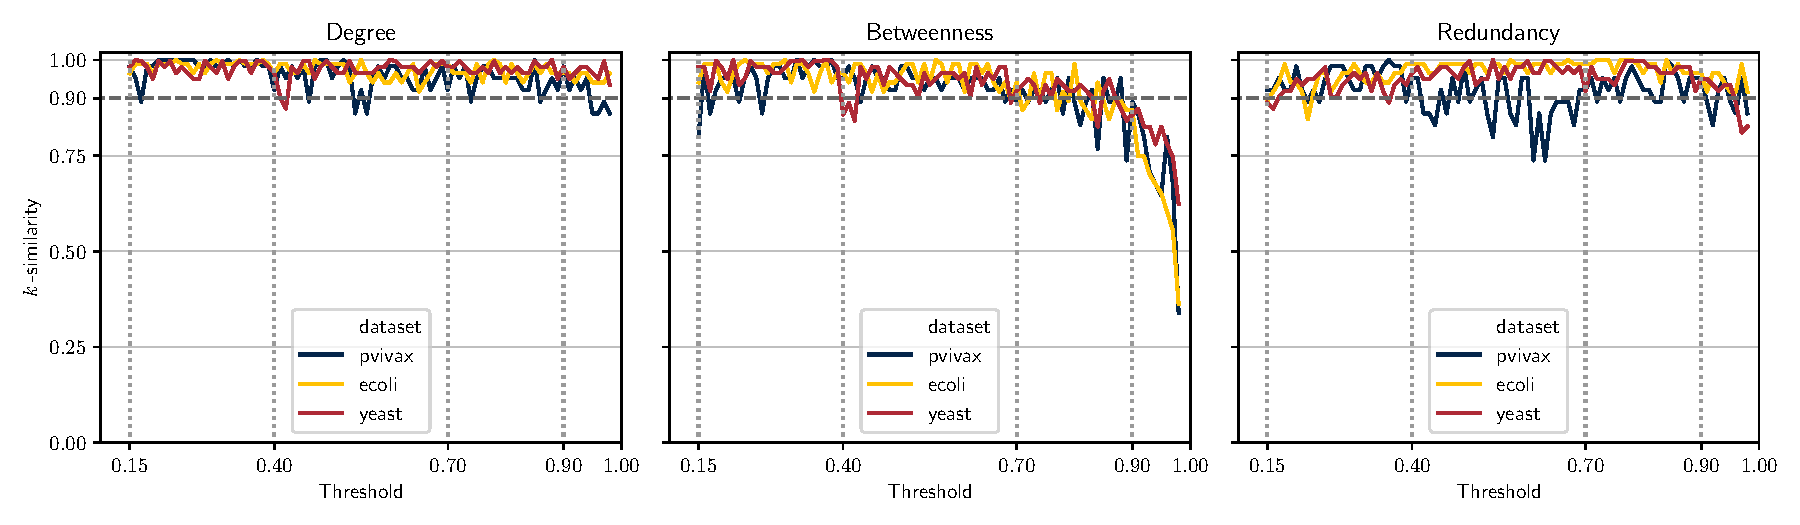
\includegraphics[align=t,width=\linewidth]{plot_rank_similarity_graffs.pdf}
    \end{enumerate}
    \vspace*{-0.6cm}

    \caption{Comparison of $k$-similarity plots from The Paper~(a) and from values calculated by \graffs~(b).
        Each plot shows $k$-similarity between ranks of graphs derived from protein networks at consecutive thresholds.
    The three chosen metrics \texttt{Degree}, \texttt{Betweenness}, \texttt{Redundancy} demonstrate that values obtained by \graffs closely match those from The Paper.}
    \label{fig:plot_rank_similarity}
\end{figure}

\begin{figure}
    \begin{enumerate}
        \item[(a)] 
\includegraphics[scale=1.05]{plot_relaxed_similarity_papertop.pdf}\\
        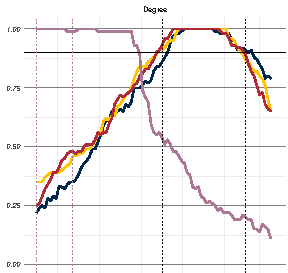
\includegraphics[scale=1.05,trim={0 0.8mm 0 0},clip]{plot_relaxed_similarity_paper_degree.pdf}\hspace*{0.2mm}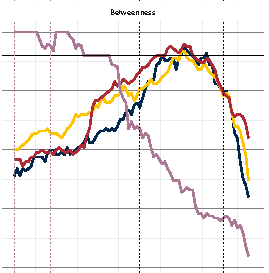
\includegraphics[scale=1.05,trim={0 0.3mm 0 0},clip]{plot_relaxed_similarity_paper_betweenness.pdf}\hspace*{-0.45mm}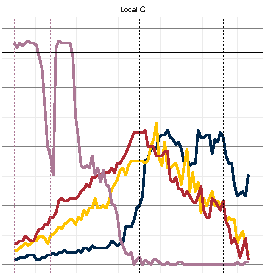
\includegraphics[scale=1.05,trim={0 0.8mm 0 0},clip]{plot_relaxed_similarity_paper_localc.pdf}\\
        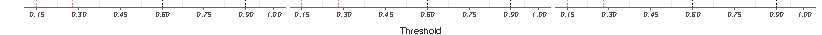
\includegraphics[scale=1.05]{plot_relaxed_similarity_paperbottom.pdf}
        \vspace*{-0.6cm}
        \item[(b)] \hspace*{-0.25cm}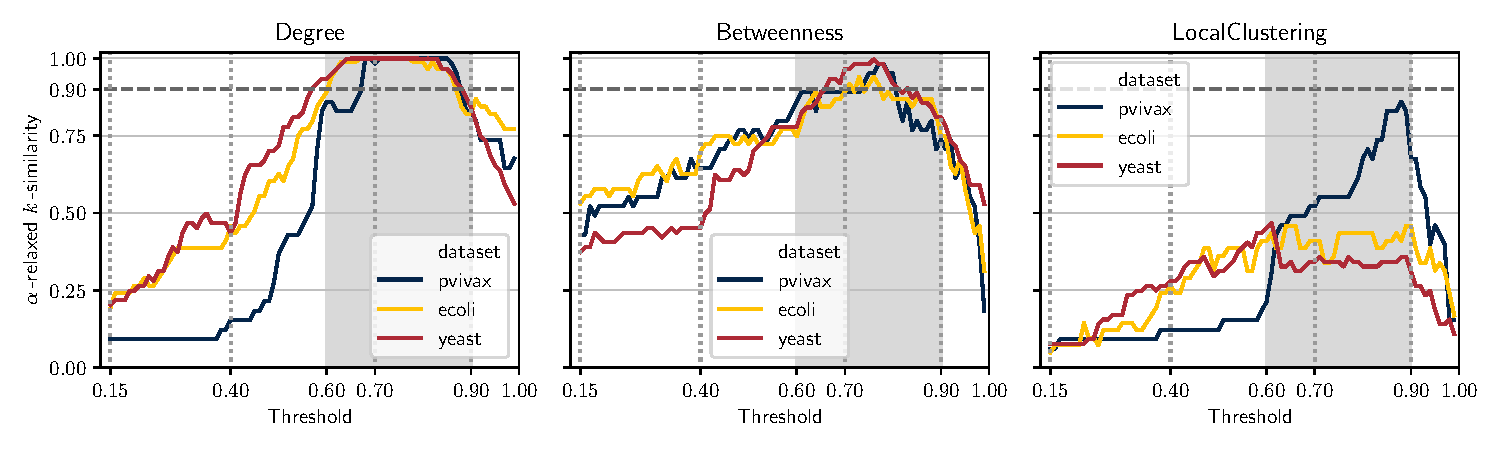
\includegraphics[align=t,width=\linewidth]{plot_relaxed_similarity_graffs.pdf}
    \end{enumerate}
    \vspace*{-0.6cm}

    \caption{Comparison of $\alpha$-relaxed $k$-similarity plots from The Paper~(a) and \graffs~(b).
        Each plot shows relaxed similarity between overall rank and ranks at individual thresholds.
    The three chosen metrics \texttt{Degree}, \texttt{Betweenness}, \texttt{LocalClustering} demonstrate that values obtained by \graffs closely match those from The Paper.}
    \label{fig:plot_relaxed_similarity}
\end{figure}

\afterpage{\clearpage}

\autoref{fig:plot_rank_similarity} shows $k$-similarity of each pair of graphs at consecutive thresholds, along with plots of the same data from The Paper.
The $k$-similarity values are used for calculating \texttt{RankContinuity}, which is equal to the proportion of such pairs of consecutive graphs whose $k$-similarity is above the $0.9$ threshold).

\autoref{fig:plot_relaxed_similarity} shows $\alpha$-relaxed $k$-similarity between overall ranking and rankings of graphs at individual thresholds.
$\alpha$-relaxed $k$-similarity is used for calculating \texttt{RankIdentifiability}, which is equal to the minimum similarity value within the $\left[ 0.6, 0.9 \right]$ confidence interval.

The visual plots of the three chosen metrics in each case demonstrate that \graffs's similarity values match those of The Paper closely, in both $k$-similarity and $\alpha$-relaxed $k$-similarity.

\section{Validation of random edge deletion}

\begin{wrapfigure}{R}{0.5\textwidth}
    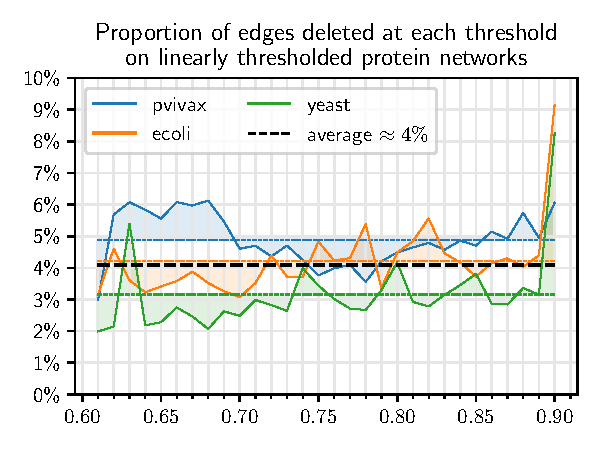
\includegraphics[width=\linewidth]{plot_edge_deletion_per_step.pdf}
    \vspace*{-0.5cm}
    \caption{Proportion of deleted edges in 3 protein network (around $4\%$ at each threshold)}
    \label{fig:plot_edge_deletion_per_step}
\end{wrapfigure}


Randomly deleting a small subset of edges allows us to evaluate robustness of metrics on unscored graphs.
The purpose of the \texttt{random-edges} experiment is to justify reliability and accuracy of this approach, comparing robustness results of the same metrics, on the same datasets, just with a different graph-generating method.

Taking distribution of confidence scores from \autoref{fig:histogram_edges} and differentiating its right-to-left accumulation function results in \autoref{fig:plot_edge_deletion_per_step}.
This shows that the relative amount of edges deleted when increasing the threshold in $0.01$ increments, is $4\%$ in average.
Thus, I set $\delta=0.04$ (proportion of edges to delete) in the random edge deletion algorithm (see \autoref{eq:edge_removing_generator}).
To make this graph generator work on unscored graphs comparably to scored graphs as in the previous experiment, I also set the \textsl{initial threshold} of each scored graph to the confidence of $0.6$.

Also note that the rank continuity metric (definition~\ref{def:rank_continuity}) is only applicable to scored datasets, so will not be computed in this experiment.

The experiment was set up using the following commands:
% @formatter:off
\begin{lstlisting}[language=bash]
graffs dataset download-demos
graffs generator create --name random04 --method removing-edges --params 0.04,600 -n 31 --seed 7
graffs experiment create --name random-edges --datasets pvivax,ecoli,yeast --generator random04 --metrics Betweenness,Degree,Ego1Edges,Ego2Nodes,LocalClustering,PageRank,Redundancy --robustnessMeasures RankIdentifiability,RankInstability
graffs experiment run --name random-edges
\end{lstlisting}
% @formatter:on

\begin{figure}
    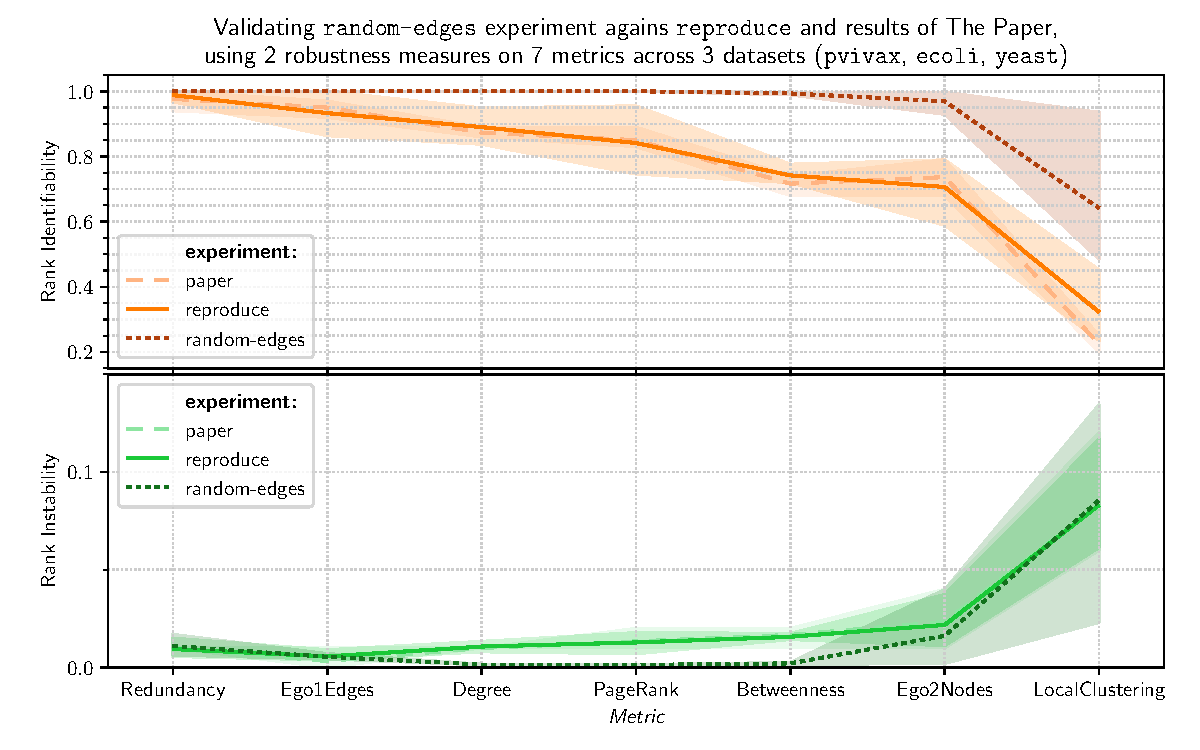
\includegraphics[width=\linewidth]{plot_random_edges.pdf}
    \caption{Validation of the \texttt{random-edges} experiment against \texttt{reproduce} and results of The Paper, using RankIdentifiability and RankInstability (displayed separately) on 7 metrics across 3 datasets.
    Thin lines inside each color band band show robustness of individual datasets, and the thick line shows the average robustness across the 3 datasets.
    Each line style (solid, long dashes, short dashes) corresponds to results obtained from different experiment or source.}
    \label{fig:plot_random_edges}
    \footnotesize
    \begin{flushleft}
        High values of RankIdentifiability mean high \textsl{robustness}, whereas high values of RankInstability mean low \textsl{robustness}.
        Metrics are sorted from left to right by their decreasing combined robustness.
    \end{flushleft}
\end{figure}


Results are shown in \autoref{fig:plot_random_edges}.
We can see that RankInstability is able to flag both \texttt{Ego2Nodes} and \texttt{LocalClustering} metrics as relatively unstable, whereas Rank Identifiability only identified \texttt{LocalClustering} as unstable, and moreover with high variance among the datasets.


\section{Extending to unscored datasets}

Having validated that randomly removing edges is a reasonable method for generating small perturbations in unscored graphs, we can now proceed to evaluating robustness of multiple metrics on multiple interesting datasets.
I have chosen the following datasets, considering mainly their size (number of nodes and density; due to associated computational cost), and supposed structure.

\begin{description}
    \item[airports]\ Airport–airport flights in the US in 2010~\cite{konect:2016:opsahl-usairport,konect:opsahl11}, from KONECT~\cite{Kunegis2013}
    \item[citation]\ High-energy physics theory citation network~\cite{LeskovecGraphsTimeDensification2005,GehrkeOverview2003KDD2003}, from SNAP Datasets~\cite{Large2016}
    \item[collab]\ Collaboration network of Arxiv General Relativity category~\cite{LeskovecGraphEvolutionDensification2007}, SNAP Datasets
    \item[facebook]\ Social circles (friends) from Facebook~\cite{NIPS2012_4532}, from SNAP Datasets
    \item[internet]\ Internet topology network of autonomous systems~\cite{konect:zhang05,konect:2016:topology}, from KONECT
\end{description}

\todo{mention licenses of datasets, and include them on download}


The experiment using these datasets is set up as follows:
% @formatter:off
\begin{lstlisting}[language=bash]
graffs dataset download-demos
graffs experiment create --name unscored --generator random04 \
    --datasets airports,citation,collab,facebook,internet \
    --metrics Betweenness,Degree,Ego1Edges,Ego2Nodes,LocalClustering,PageRank,Redundancy \
    --robustnessMeasures RankIdentifiability,RankInstability,RankContinuity
graffs experiment run --name unscored
\end{lstlisting}
% @formatter:on

\begin{figure}
    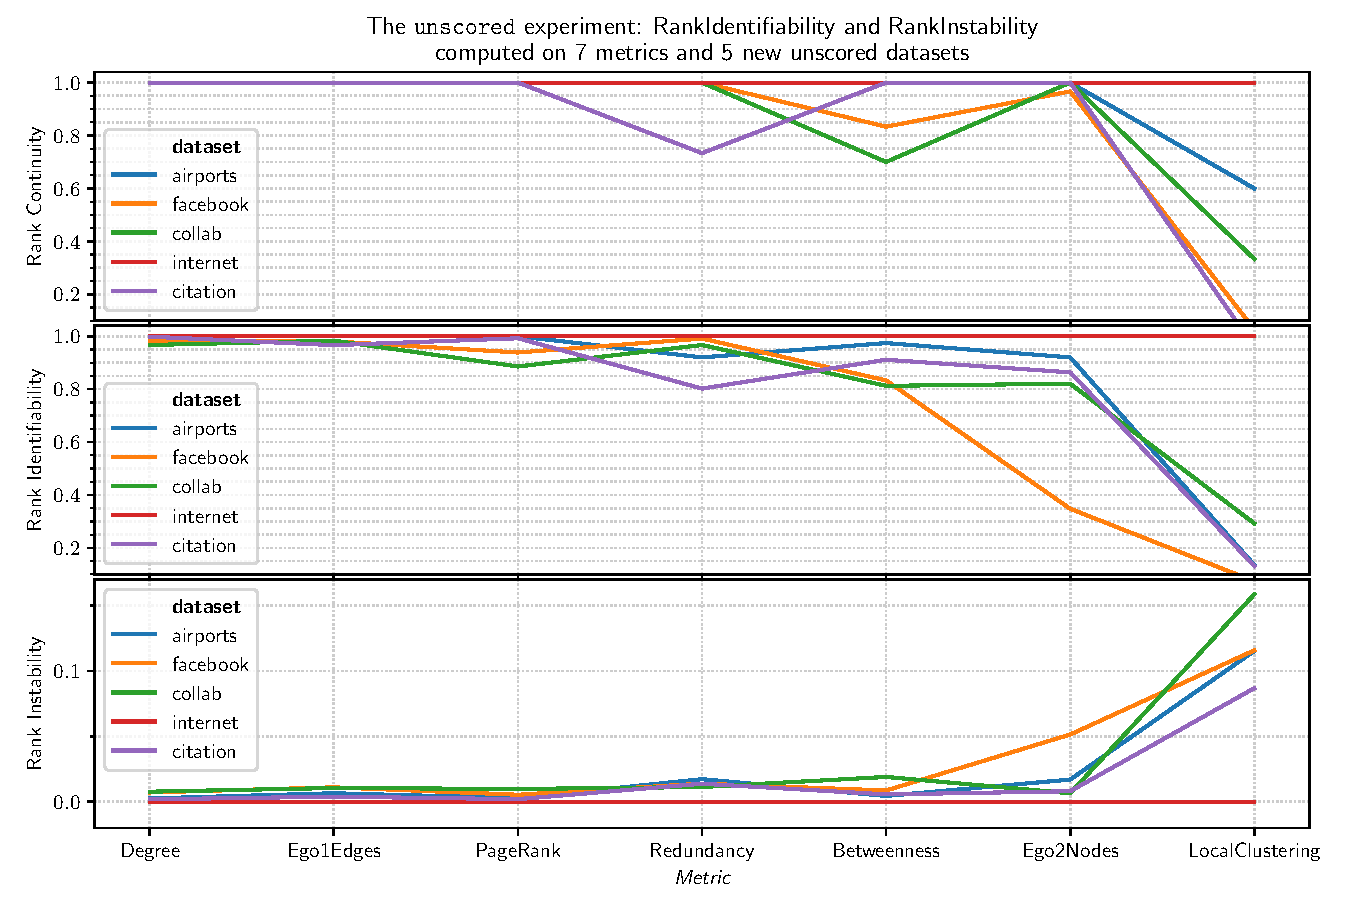
\includegraphics[width=\linewidth]{plot_unscored.pdf}
    \vspace*{-0.6cm}
    \caption{Evaluating RankContinuity, RankIdentifiability and RankInstability on 5 new unscored datasets, generating graphs by randomly deleting $4\%$ of edges.}
    \label{fig:plot_unscored}
    \footnotesize\justify\vspace{-0.4\baselineskip}
    High values of RankContinuity and RankIdentifiability mean high robustness, whereas high values of RankInstability mean low robustness.
    Metrics are sorted from left to right by their decreasing combined robustness.
\end{figure}


\autoref{fig:plot_unscored} shows 2 robustness measures evaluated on the 7 metrics using 5 unscored datasets.
Overall, the tendency of robustness measures identify the key results from previous experiments: metrics \texttt{Degree}, \texttt{Ego1Edges}, and \texttt{Redundancy} are stable on all datasets.
The \texttt{facebook} dataset has lower RankIdentifiability of \texttt{Betweenness} and \texttt{Ego2Nodes} metric, and most of the datasets apart from \texttt{internet} have lower values of both robustness measures of the \texttt{LocalClustering} metric.


\section{Performance}

The following plots compare the time it took to evaluate the experiments: \texttt{reproduce}, \texttt{random-edges}, \texttt{unscored}; and the time spent on evaluating each metric.

I ran the experiments on a computing server running \textsl{Ubuntu 18}, using \textsl{4x 8-Core AMD Opteron 6128} with 16 MiB L2 cache (32 cores in total), and 128 GiB RAM installed.

\todo{include plots}

% reproduce
%Generate graphs            : 51s
%Evaluate metrics - run     : 38m 46s
%Robustness - compute       : 10s


\section{Releasing \graffs}

\subsection{Licensing}
